\documentclass{article}

\usepackage{a4}
\usepackage{amsmath}
\usepackage{amssymb}
\usepackage{ctex}
\usepackage{booktabs}
\usepackage{graphicx}
\usepackage{subfigure}
\usepackage{subcaption}
\usepackage{float}
\usepackage{hyperref}
\usepackage{xurl}
\usepackage{enumitem}
\usepackage{array}
\usepackage{longtable}
\usepackage{multirow}

\hypersetup{colorlinks=true,linkcolor=black,urlcolor=blue,citecolor=black}
\setlist[itemize]{nosep,leftmargin=1.8em}
\setlist[enumerate]{nosep,leftmargin=1.8em}
\captionsetup{font=small}

\title{计算机组成原理 \\ 实验1 数据运算：定点加法}
\author{鲁昕宁 2414015}
\date{\today}

\begin{document}

\maketitle
\begin{center}
    \url{https://github.com/SidneyLu/Computer-Organization-and-Design-NKU-CS/tree/master/lab1}
\end{center}

\newpage

\section{实验目标}
参考实验指导手册第一次的加法器实验，完成对加法器的改进：

\begin{itemize}
\item 将原始的两个32位数的加法器，改进成4个32位数的加法器。
\item 修改testbench模块，通过波形仿真验证改进加法器的正确性。
\item 修改display模块和约束文件，通过上试验箱验证加法器正确性。
\end{itemize}

\section{实验原理}
\subsection{四操作数定点加法}
本实验在原有两操作数加法器基础上，将输入扩展为 4 路 32 位加数和 1 位输入进位：
\[
\{cout,result\}=operand1+operand2+operand3+operand4+cin
\]
其中 \verb|result| 为低 32 位结果，\verb|cout| 为高位进位输出（保持与原实验接口一致）。

\subsection{显示与交互机制}
顶层模块 \verb|adder_display.v| 通过触摸屏输入 32 位数据，通过拨码开关选择写入目标操作数，并在屏幕固定区域显示 4 个加数与结果；\verb|sw_cin| 作为输入进位，\verb|led_cout| 显示输出进位。

\begin{table}[H]
\centering
\caption{input\_sel 与输入目标映射}
\begin{tabular}{c|c}
\toprule
\textbf{input\_sel} & \textbf{写入对象} \\
\midrule
00 & adder\_operand1 \\
01 & adder\_operand2 \\
10 & adder\_operand3 \\
11 & adder\_operand4 \\
\bottomrule
\end{tabular}
\end{table}

\begin{figure}[h!]
\centering
    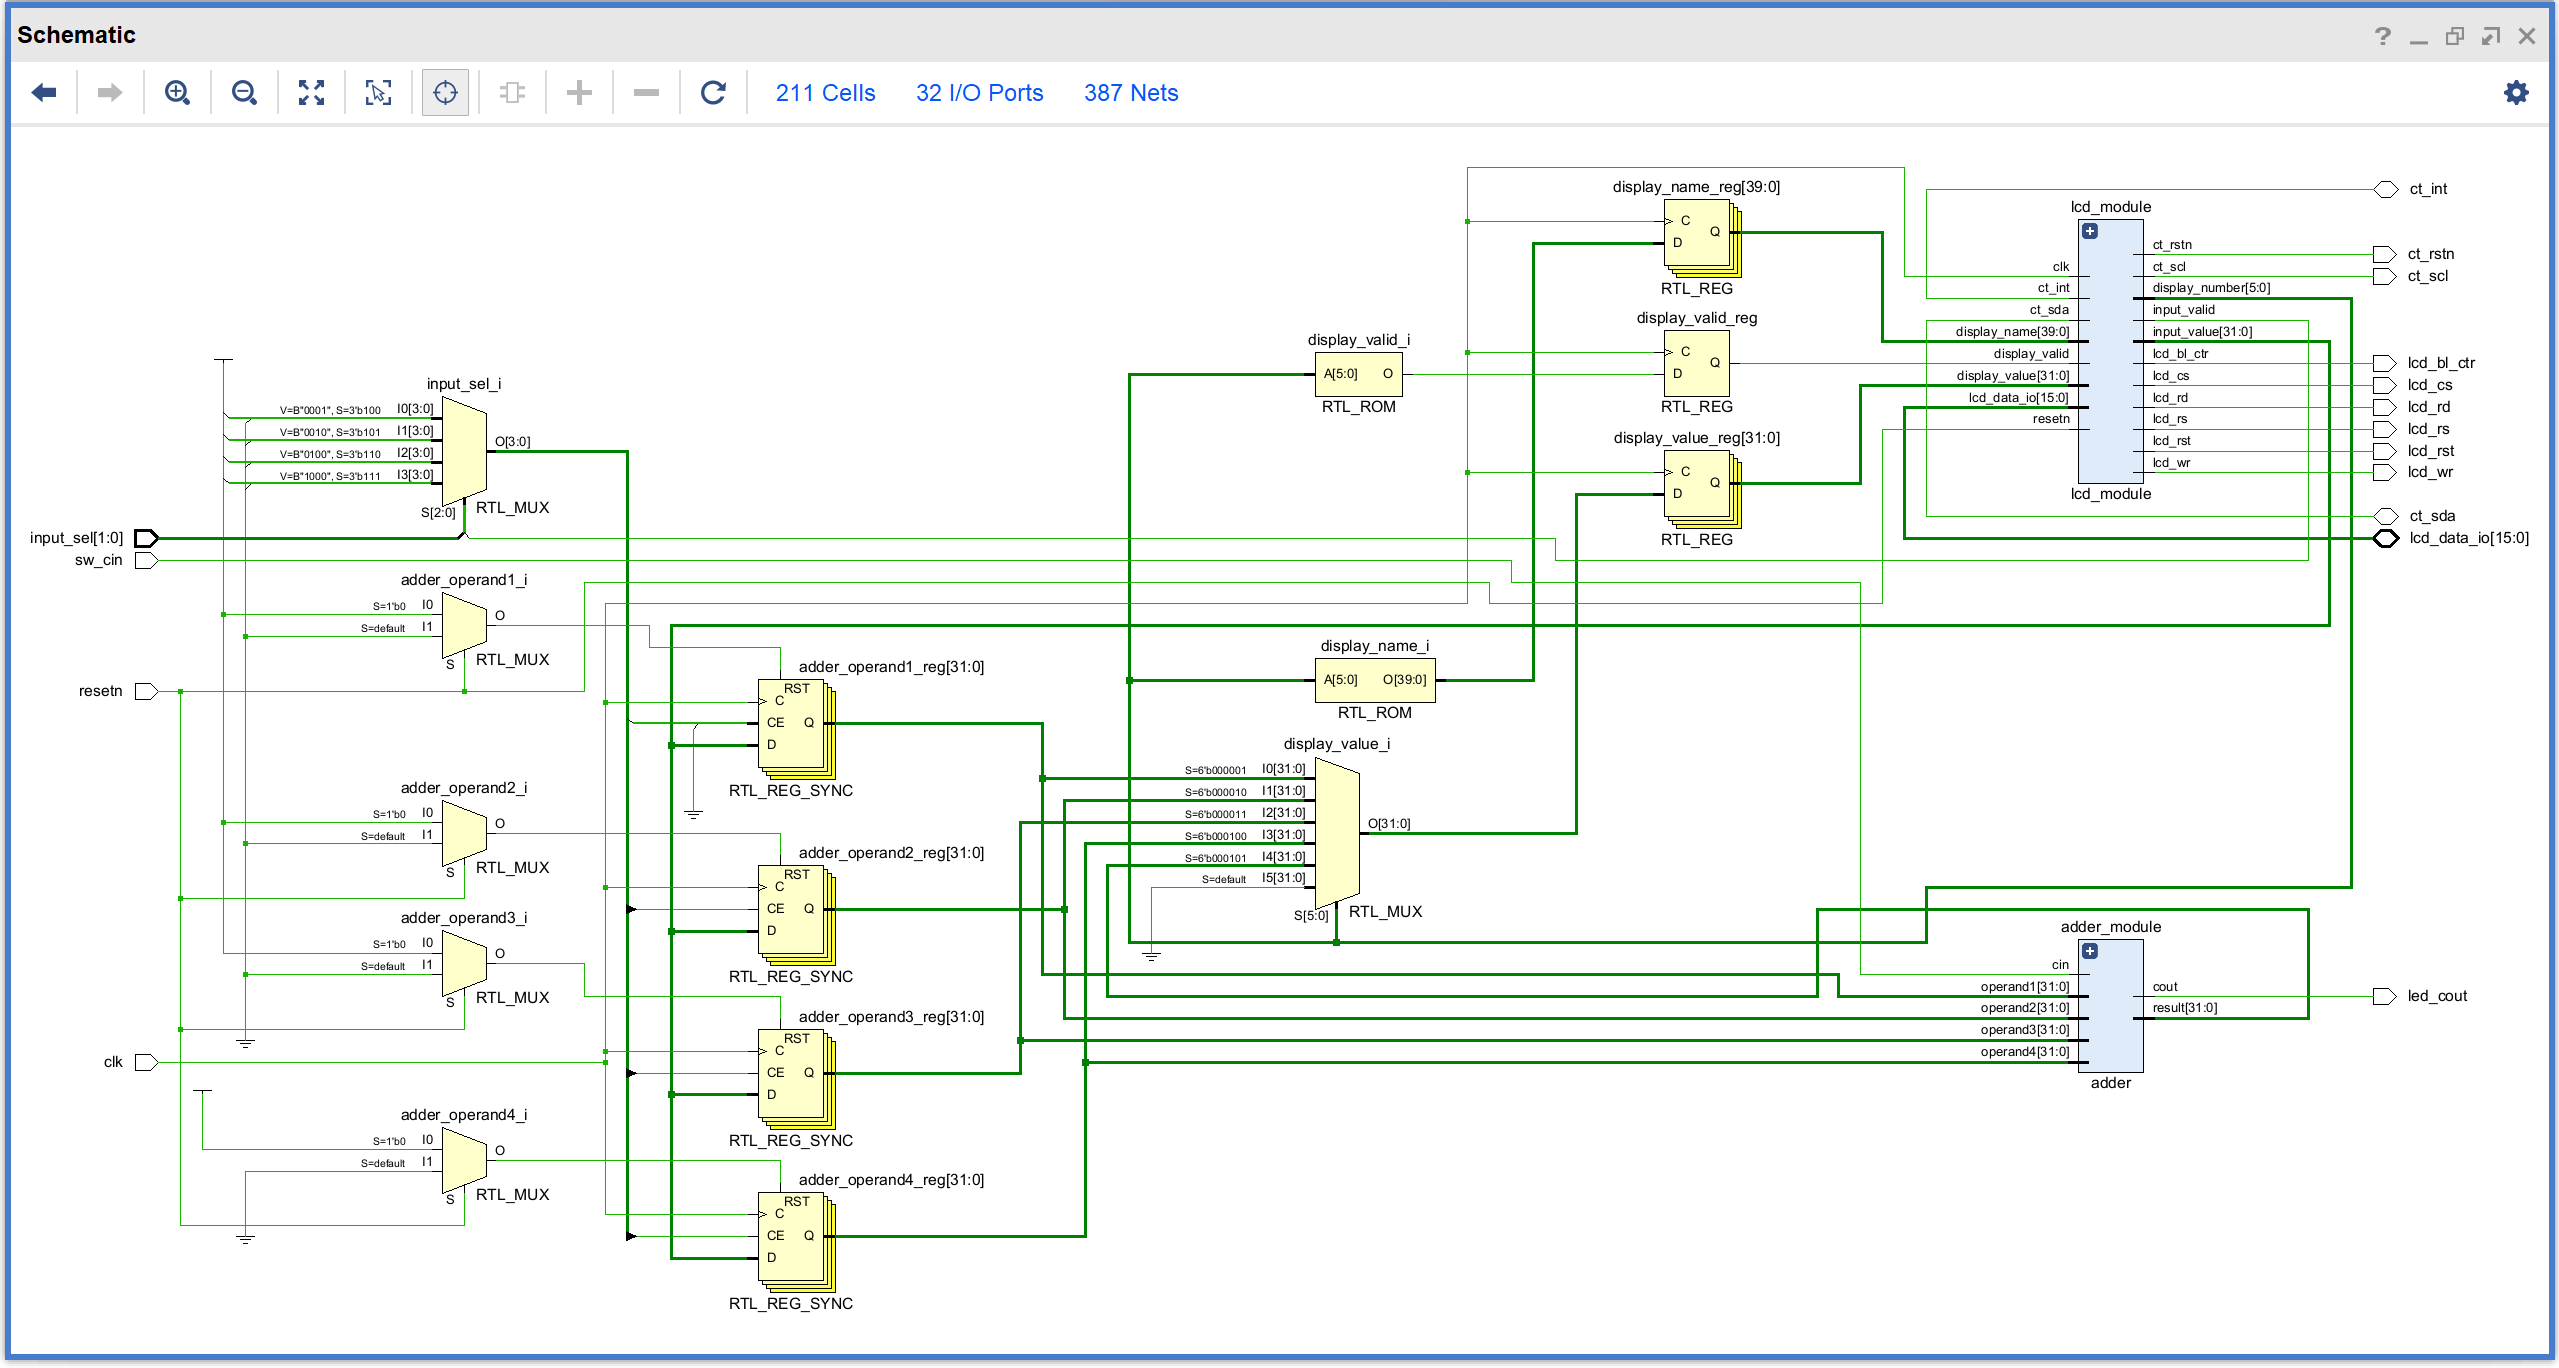
\includegraphics[width=0.8\textwidth]{schematic.png}
    \caption{加法器原理图}
    \label{fig:schematic}
\end{figure}

\section{实验过程}
\subsection{源码修改}
Verilog 源码位于 \verb|lab1/lab1.srcs|，关键修改片段如下。

\paragraph{1) \texttt{sources\_1/new/adder.v}（四操作数加法）}
\begin{verbatim}
module adder(
    input  [31:0] operand1,
    input  [31:0] operand2,
    input  [31:0] operand3,
    input  [31:0] operand4,
    input         cin,
    output [31:0] result,
    output        cout
    );
    assign {cout,result} = operand1 + operand2 +
                           operand3 + operand4 + cin;
endmodule
\end{verbatim}

\paragraph{2) \texttt{sources\_1/new/adder\_display.v}（输入扩展与显示扩展）}
\begin{verbatim}
input [1:0] input_sel,
...
reg  [31:0] adder_operand3;
reg  [31:0] adder_operand4;
...
else if (input_valid && input_sel==2'b10) begin
    adder_operand3 <= input_value;
end
...
else if (input_valid && input_sel==2'b11) begin
    adder_operand4 <= input_value;
end
\end{verbatim}

\begin{verbatim}
6'd3 : begin
    display_valid <= 1'b1;
    display_name  <= "ADD_3";
    display_value <= adder_operand3;
end
6'd4 : begin
    display_valid <= 1'b1;
    display_name  <= "ADD_4";
    display_value <= adder_operand4;
end
6'd5 : begin
    display_valid <= 1'b1;
    display_name  <= "RESUL";
    display_value <= adder_result;
end
\end{verbatim}

\paragraph{3) \texttt{sim\_1/new/testbench.v}（仿真激励）}
\begin{verbatim}
always #10 operand1 = $random;
always #10 operand2 = $random;
always #10 operand3 = $random;
always #10 operand4 = $random;
always #10 cin = {$random} % 2;
\end{verbatim}

\paragraph{4) \texttt{constrs\_1/new/adder.xdc}（新增管脚约束）}
\begin{verbatim}
set_property PACKAGE_PIN AC22 [get_ports input_sel[1]]
set_property PACKAGE_PIN AC23 [get_ports input_sel[0]]
set_property PACKAGE_PIN AD24 [get_ports sw_cin]

set_property IOSTANDARD LVCMOS33 [get_ports input_sel[1]]
set_property IOSTANDARD LVCMOS33 [get_ports input_sel[0]]
set_property IOSTANDARD LVCMOS33 [get_ports sw_cin]
\end{verbatim}

\subsection{仿真验证}
\begin{figure}[h!]
\centering
    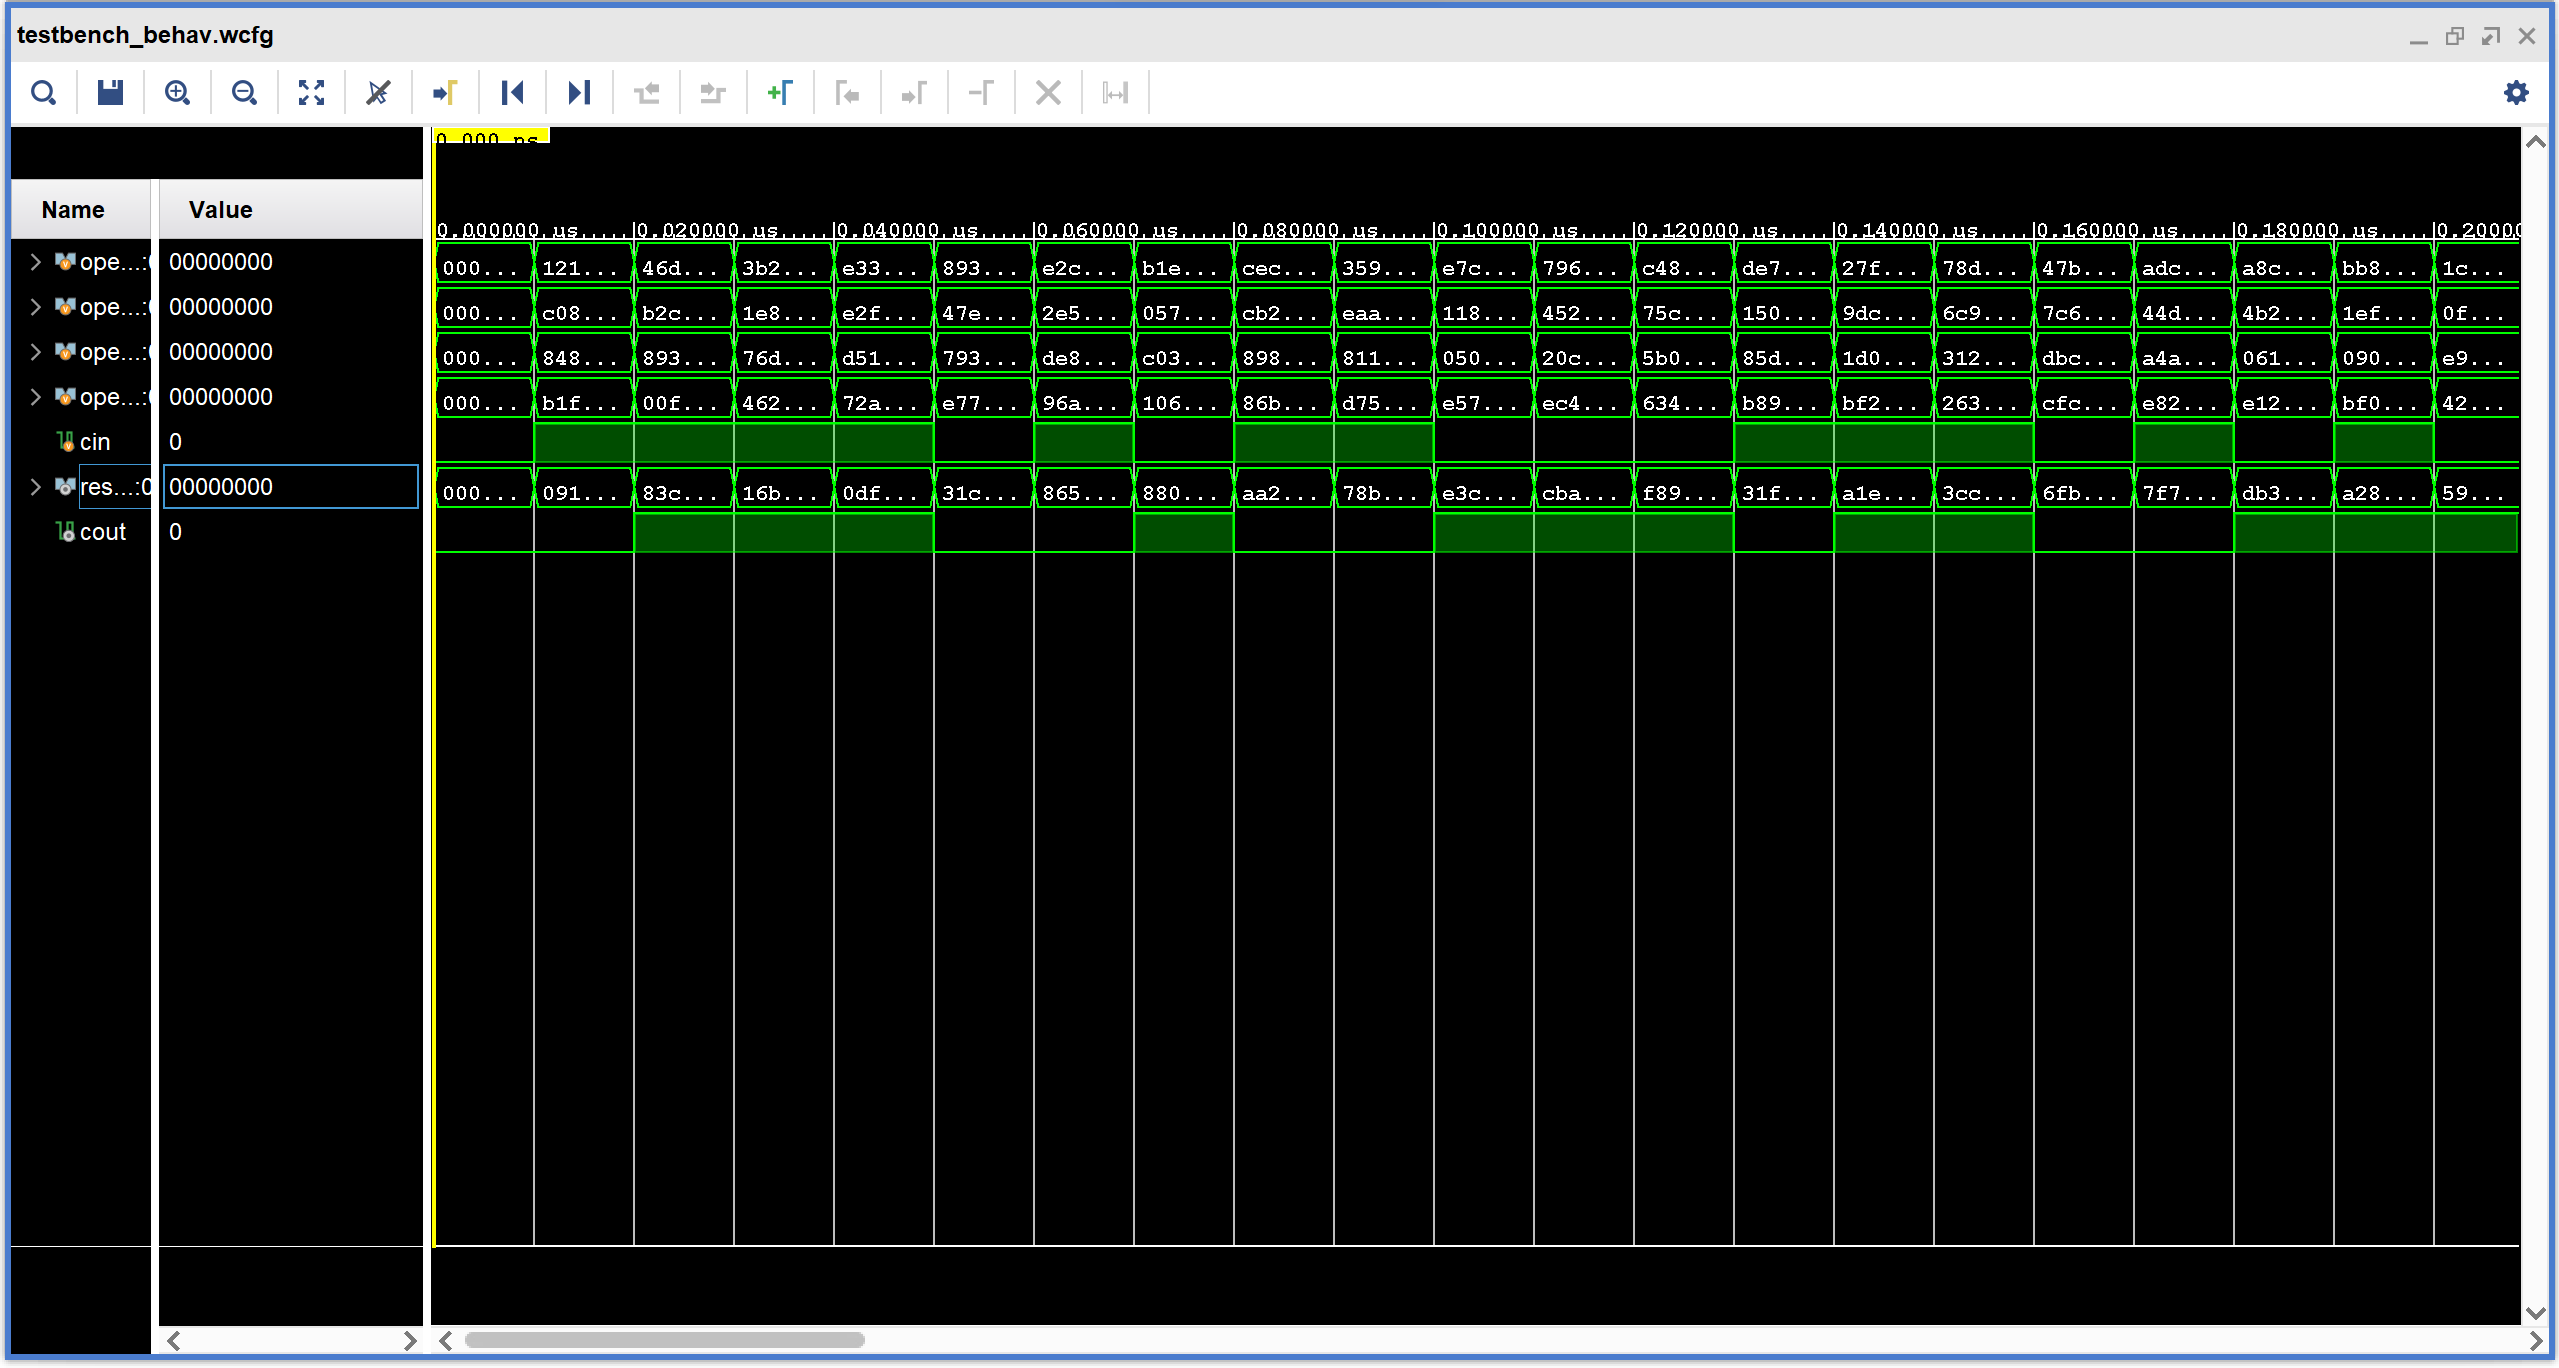
\includegraphics[width=0.8\textwidth]{simulation.png}
    \caption{加法器波形仿真}
    \label{fig:simulation}
\end{figure}
仿真中 4 路操作数每 10ns 随机变化，\verb|result| 与 \verb|cout| 可同步响应输入变化，功能符合设计预期。

\subsection{综合与实现}
\begin{figure}[h!]
    \centering
    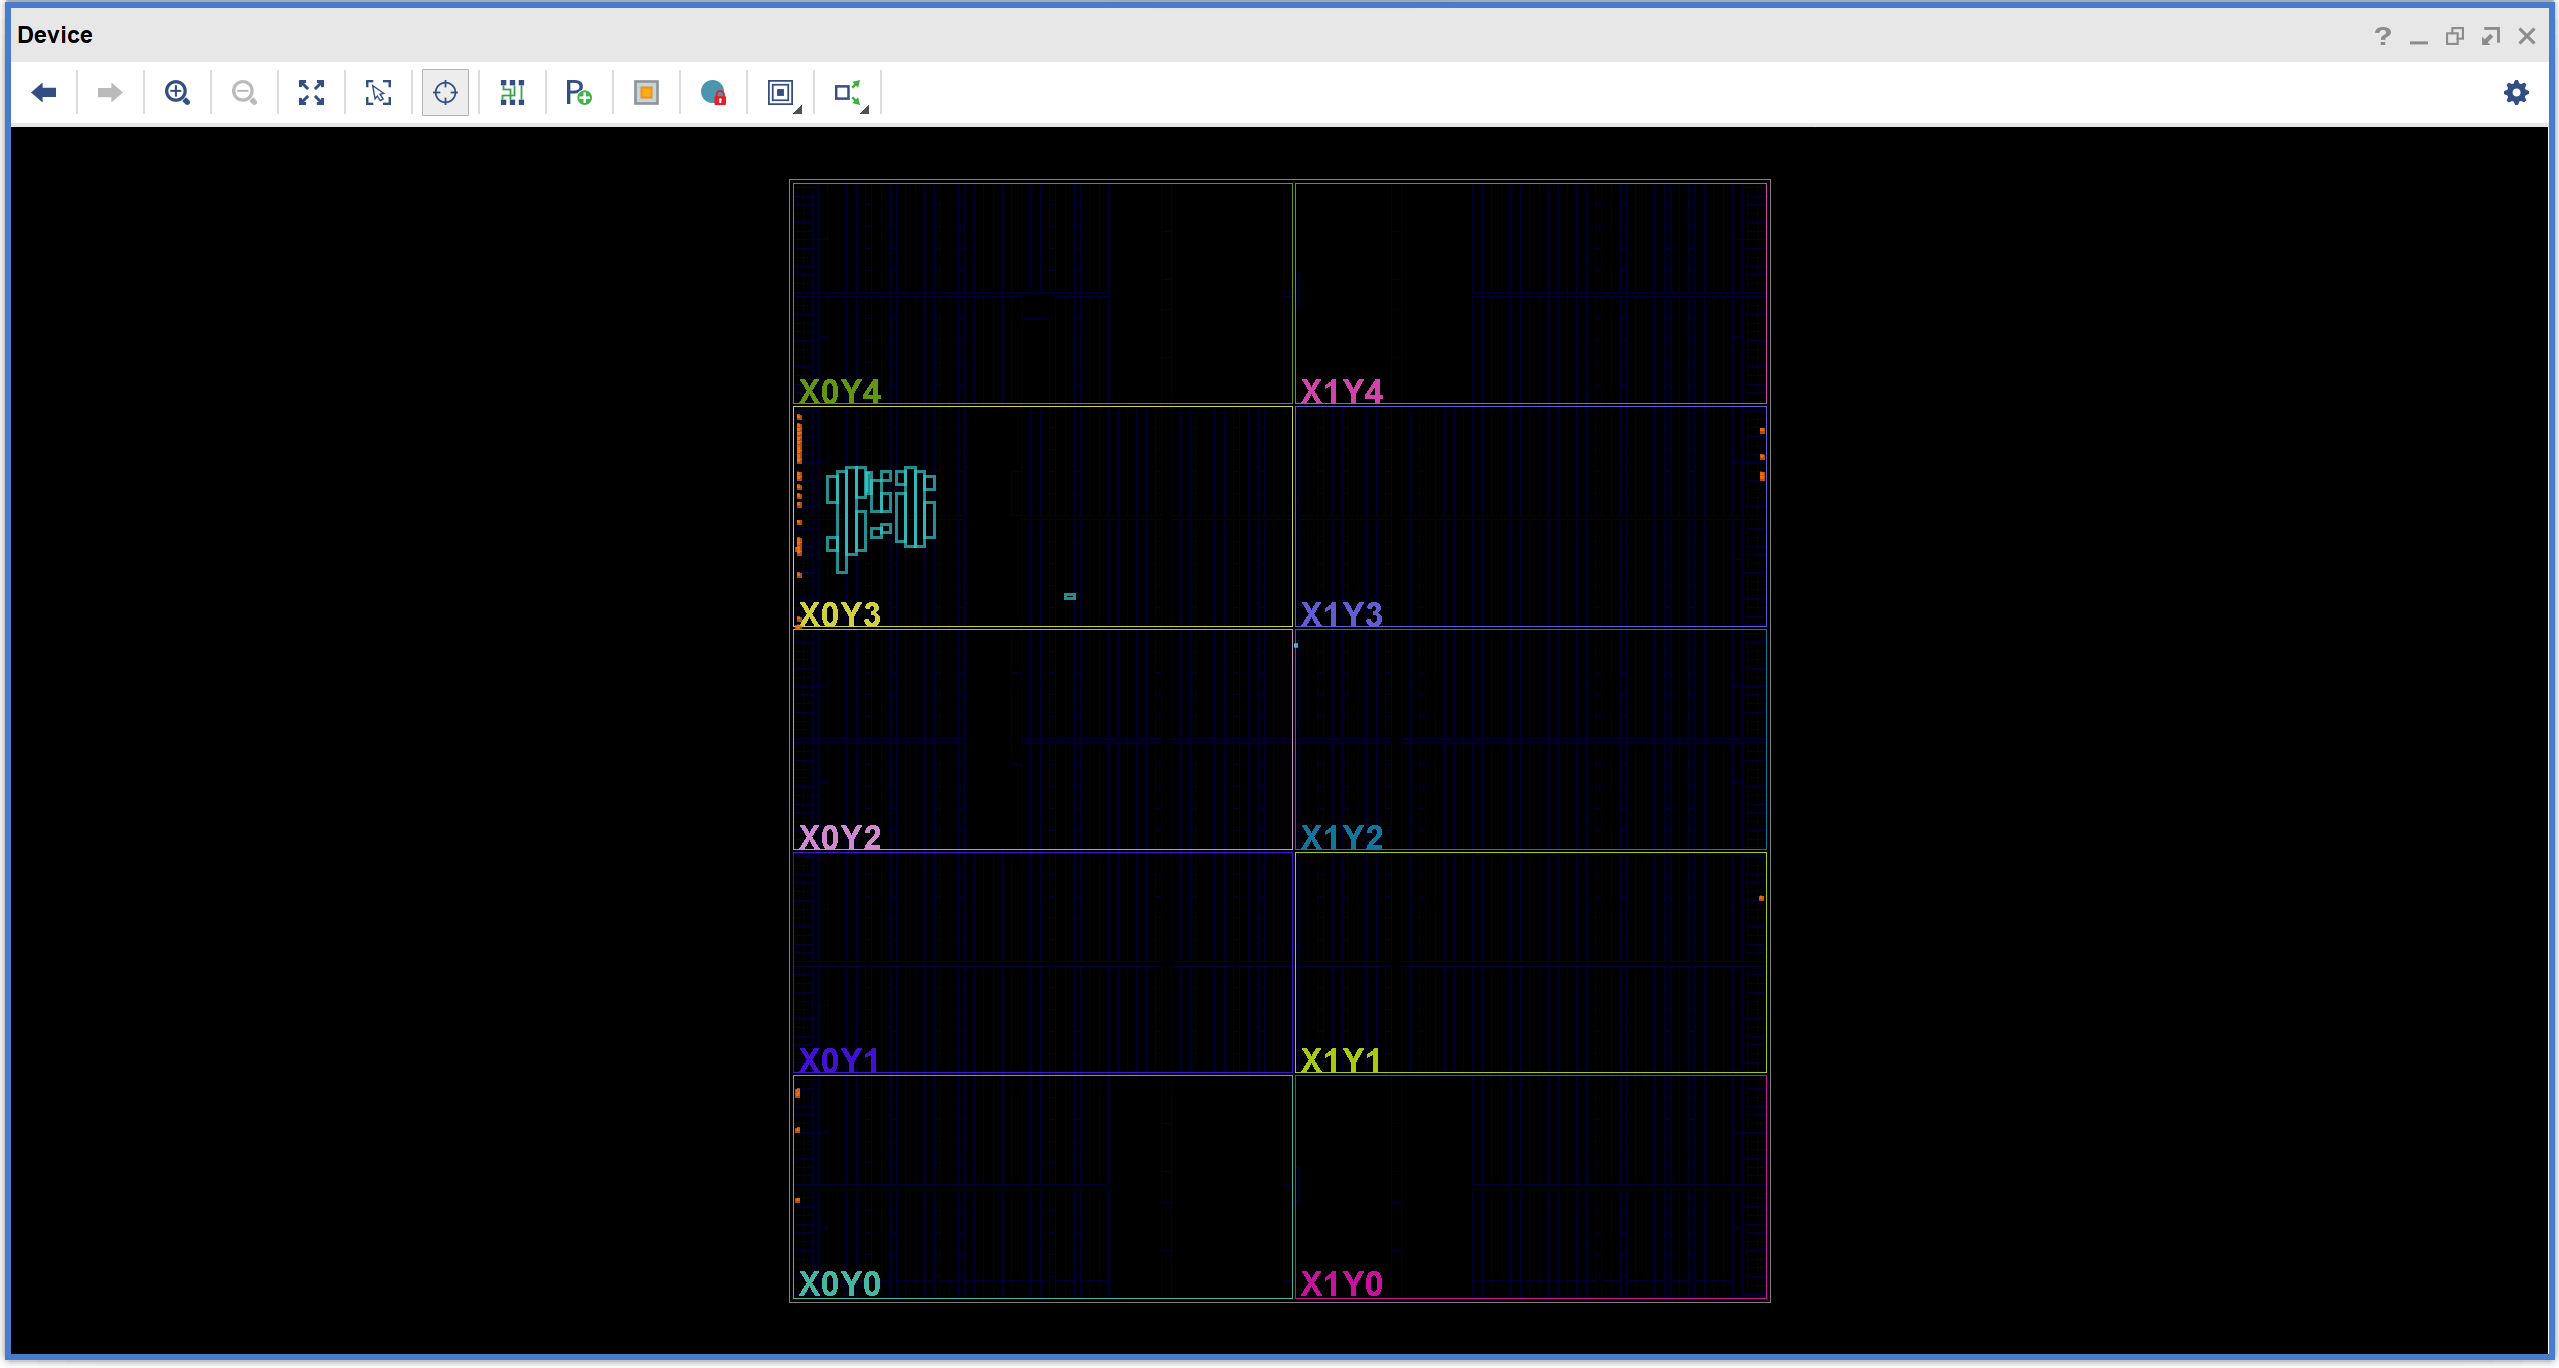
\includegraphics[width=0.8\textwidth]{implementation.png}
    \caption{加法器实现}
    \label{fig:implementation}
\end{figure}


\subsection{上板验证}
上板验证步骤如下：
\begin{enumerate}
\item 下载 \verb|adder_display.bit| 到实验箱；
\item 设置 \verb|input_sel|，通过触摸屏依次写入 4 个操作数；
\item 通过 \verb|sw_cin| 设置输入进位；
\item 观察 LCD 的 \verb|RESUL| 显示值与 \verb|led_cout| 状态是否与期望一致。
\end{enumerate}

\begin{figure}[H]
    \centering
    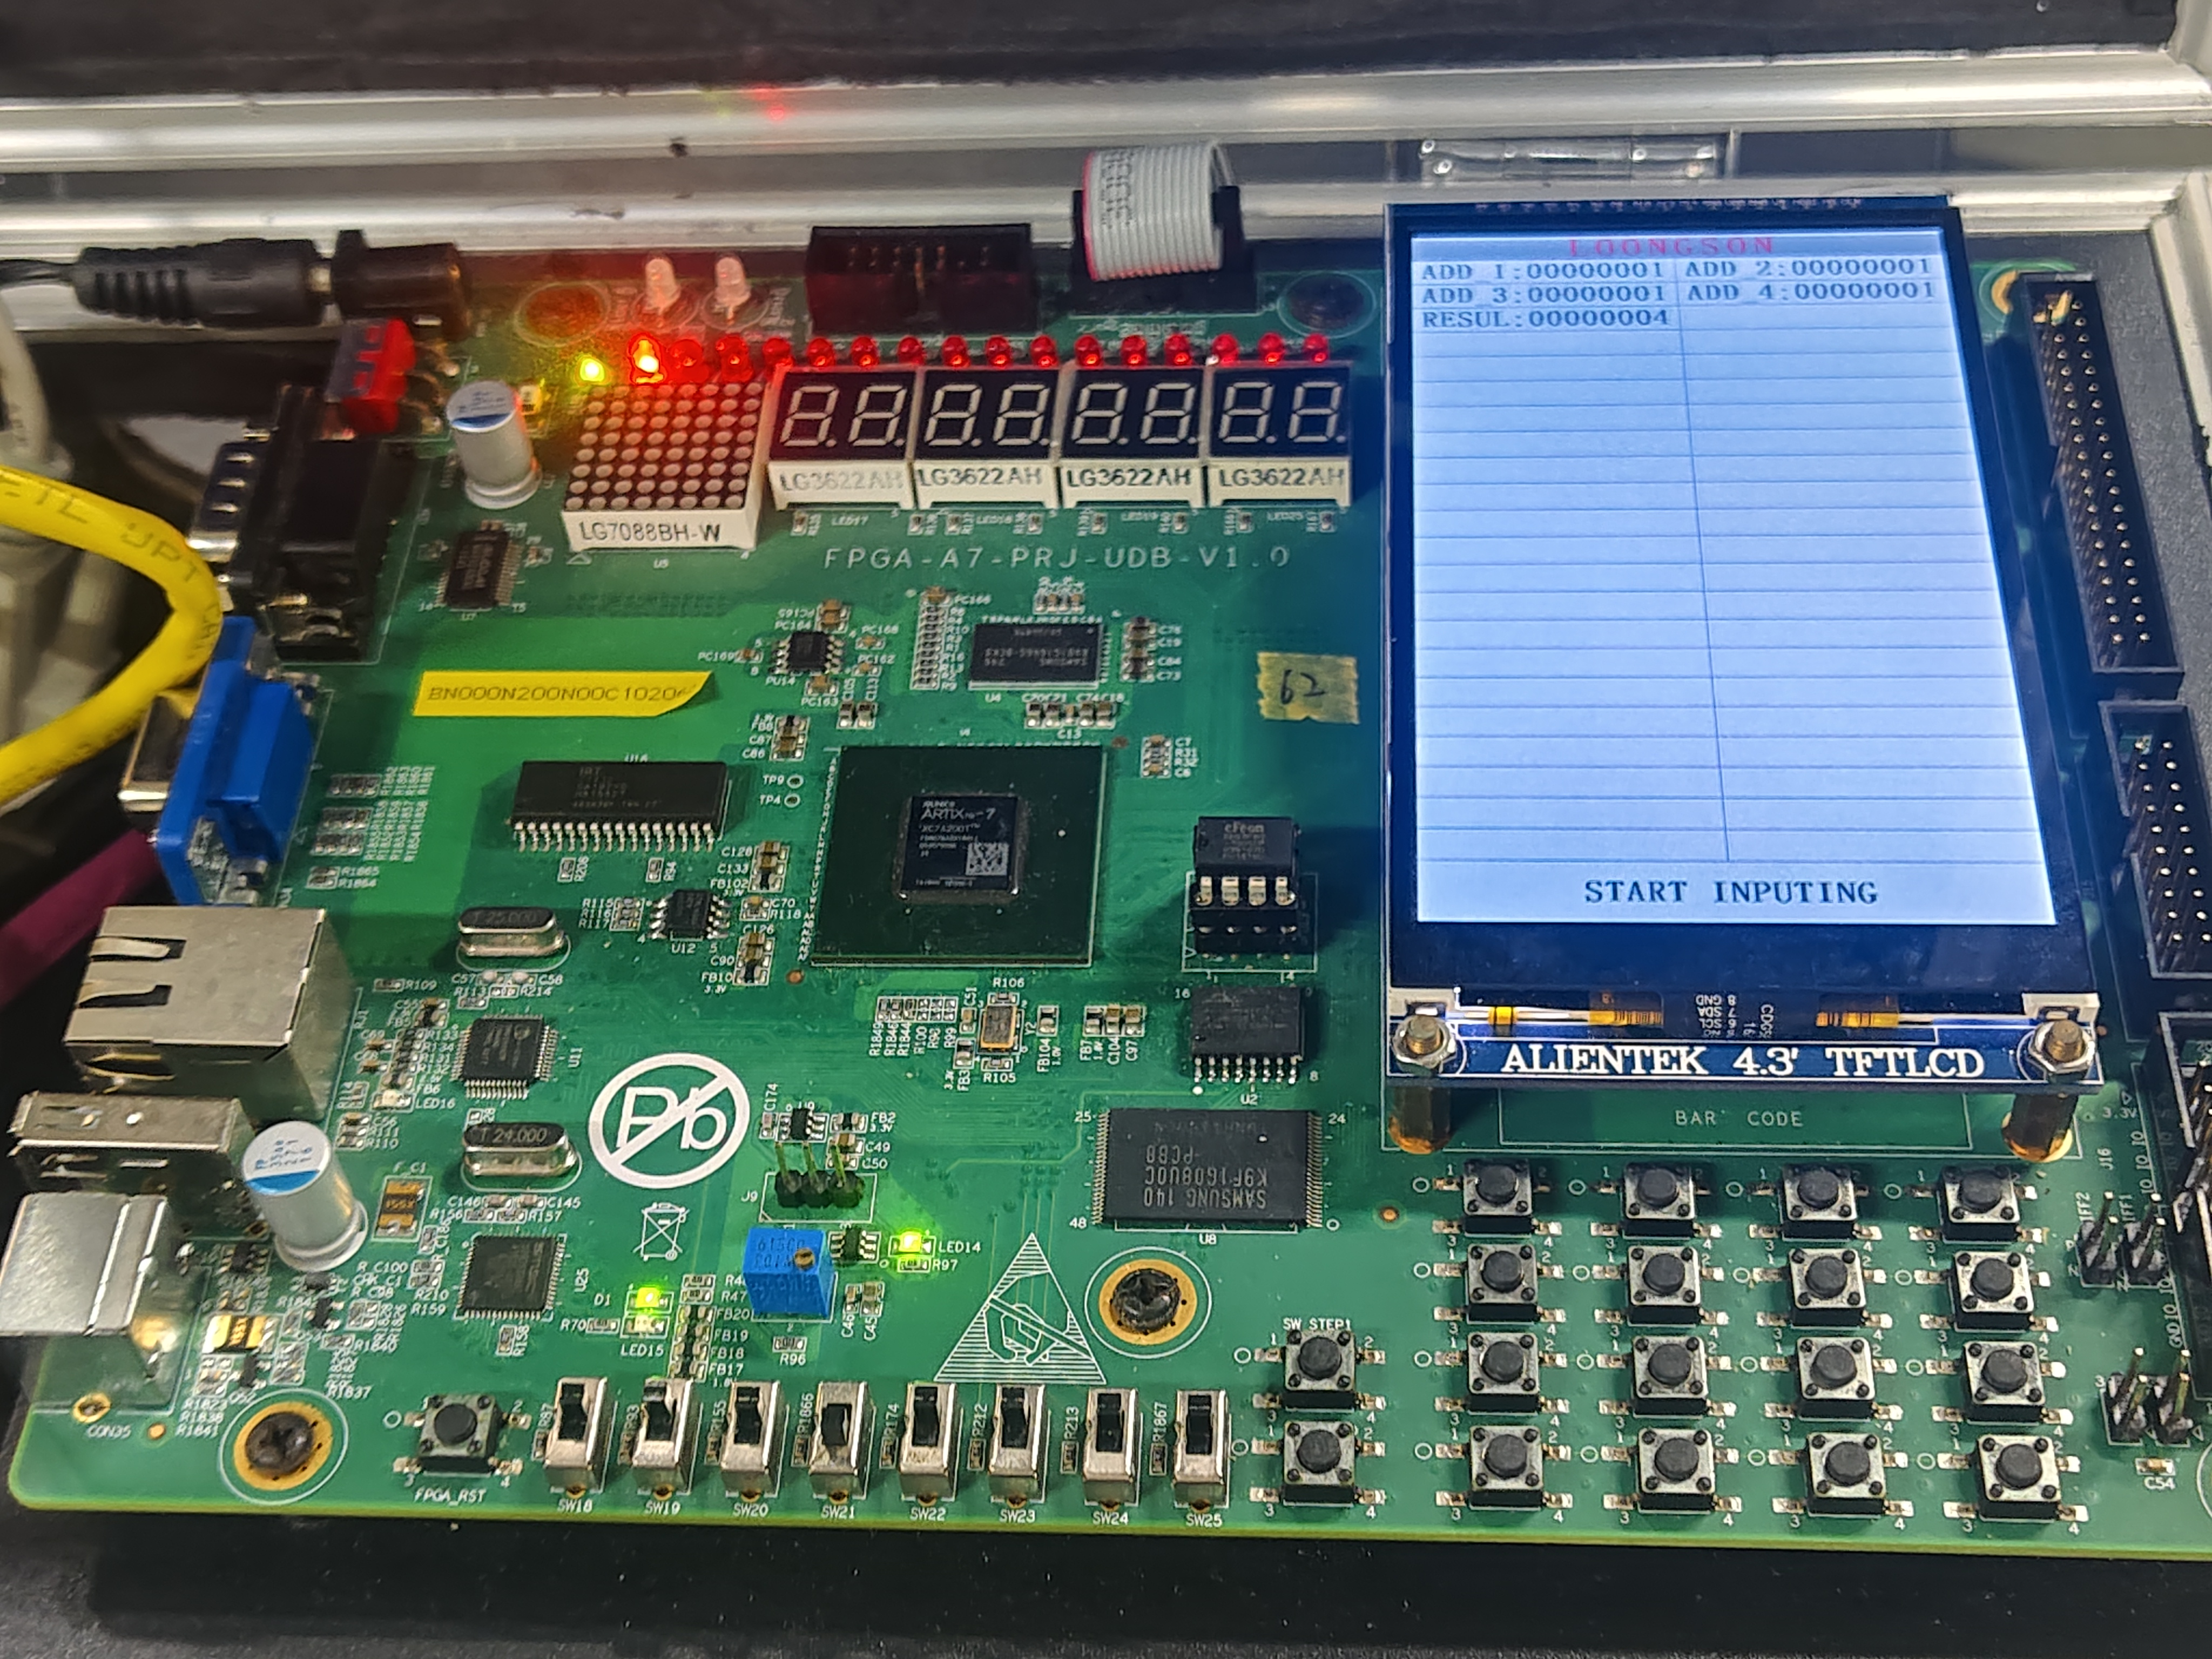
\includegraphics[width=0.8\textwidth]{onboard1.jpg}
    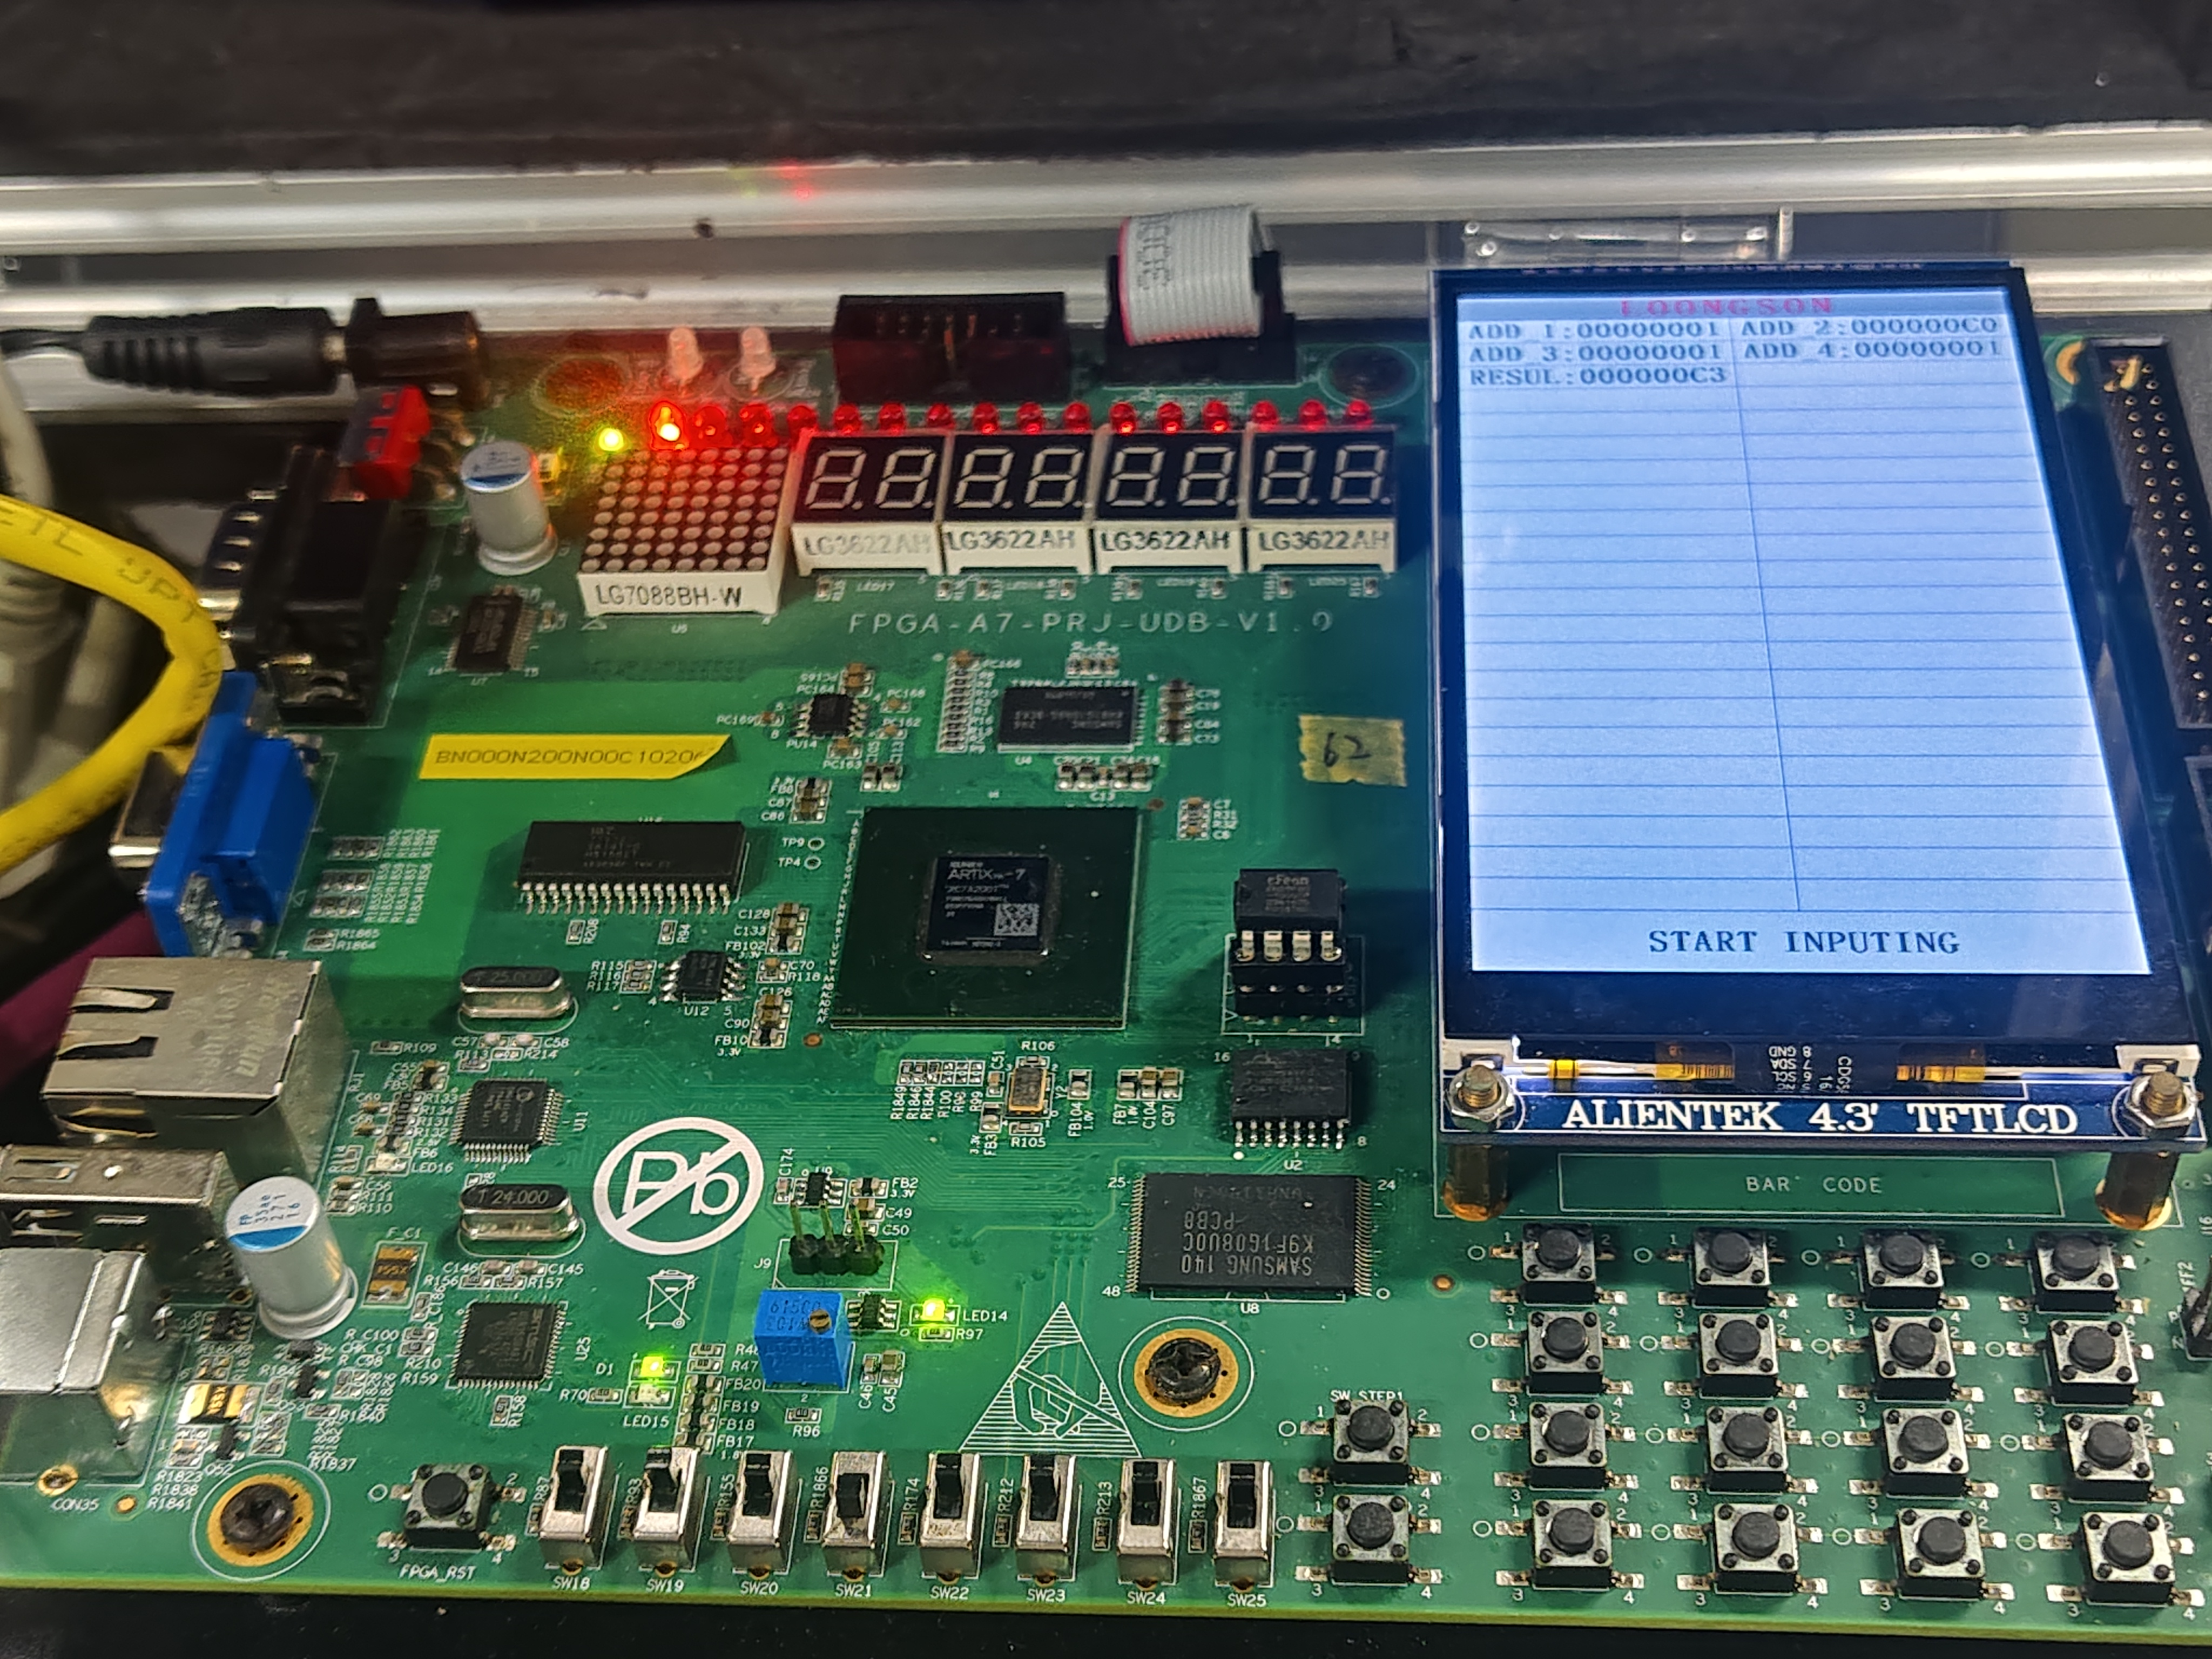
\includegraphics[width=0.8\textwidth]{onboard2.jpg}
    \caption{实验箱上板验证}
    \label{fig:board_photo}
\end{figure}

\section{实验收获}
\begin{itemize}
\item 熟悉了从“算法模块修改 $\rightarrow$ 显示交互修改 $\rightarrow$ 管脚约束修改 $\rightarrow$ 仿真/上板验证”的完整 FPGA 实验流程。
\item 掌握了组合加法器的多输入扩展方法，以及触摸屏输入、拨码开关选择和 LED 指示的协同调试方法。
\end{itemize}

\section{附：源码目录}
\begin{itemize}
\item \verb|lab1/lab1.srcs/sources_1/new/adder.v|
\item \verb|lab1/lab1.srcs/sources_1/new/adder_display.v|
\item \verb|lab1/lab1.srcs/sim_1/new/testbench.v|
\item \verb|lab1/lab1.srcs/constrs_1/new/adder.xdc|
\end{itemize}

\end{document}
